\chapter{\IfLanguageName{dutch}{Stand van zaken}{State of the art}}
\label{ch:stand-van-zaken}
\graphicspath{{../../Images/}} 
% Tip: Begin elk hoofdstuk met een paragraaf inleiding die beschrijft hoe
% dit hoofdstuk past binnen het geheel van de bachelorproef. Geef in het
% bijzonder aan wat de link is met het vorige en volgende hoofdstuk.

% Pas na deze inleidende paragraaf komt de eerste sectiehoofding.

Dit hoofdstuk bevat je literatuurstudie. De inhoud gaat verder op de inleiding, maar zal het onderwerp van de bachelorproef *diepgaand* uitspitten. De bedoeling is dat de lezer na lezing van dit hoofdstuk helemaal op de hoogte is van de huidige stand van zaken (state-of-the-art) in het onderzoeksdomein. Iemand die niet vertrouwd is met het onderwerp, weet nu voldoende om de rest van het verhaal te kunnen volgen, zonder dat die er nog andere informatie moet over opzoeken \autocite{Pollefliet2011}.

Je verwijst bij elke bewering die je doet, vakterm die je introduceert, enz. naar je bronnen. In \LaTeX{} kan dat met het commando \texttt{$\backslash${textcite\{\}}} of \texttt{$\backslash${autocite\{\}}}. Als argument van het commando geef je de ``sleutel'' van een ``record'' in een bibliografische databank in het Bib\LaTeX{}-formaat (een tekstbestand). Als je expliciet naar de auteur verwijst in de zin, gebruik je \texttt{$\backslash${}textcite\{\}}.
Soms wil je de auteur niet expliciet vernoemen, dan gebruik je \texttt{$\backslash${}autocite\{\}}. In de volgende paragraaf een voorbeeld van elk.

\textcite{Knuth1998} schreef een van de standaardwerken over sorteer- en zoekalgoritmen. Experten zijn het erover eens dat cloud computing een interessante opportuniteit vormen, zowel voor gebruikers als voor dienstverleners op vlak van informatietechnologie~\autocite{Creeger2009}.
\newpage
\section{Versiebeheer}
\subsection{Inleiding}
Versiebeheer is een belangrijk concept binnen softwareontwikkeling. Zo waren er in totaal 100 miljoen projecten op het populaire versiebeheer platform GitHub (in 2018) \autocite{Git2018}. GitHub (sinds 2018 overgenomen door Microsoft) is echter niet de enige speler op de markt. Zo is er ook nog Code Commit van Amazon en GitLab. Veel bedrijven en oplossingen spelen dus in op de behoefte voor een duidelijk en efficiënt versiebeheer systeem. Toch kan men stilstaan bij de vraag: Welke behoefte lossen deze systemen op?

Stel volgende scenario voor: Alice en Bob zijn aangenomen om te werken voor Bedrijf X. Hun eerste taak is een website ontwikkelen. Ze leggen samen alle vereisten vast, bespreken de verschillende technologieën en gaan aan de slag. Op het einde van de eerste dag hebben ze elk een verschillende pagina gemaakt en deze willen ze graag met elkaar delen.Dit kan door bijvoorbeeld via mail de bestanden door te sturen. Een andere mogelijkheid is de bestanden via fysieke hardware zoals een USB-Stick aan elkaar te geven. Het nadeel is dat de code op twee verschillende plaatsen verspreid zit. Als Bob de code die hij heeft geschreven kwijt raken, dan zal deze opnieuw moet worden geschreven. Om dit probleem te voorkomen kan men het project op een centrale server gaan opslaan. Bob en Alice zullen hun veranderingen opslaan op deze centrale server. Zo hebben ze altijd toegang tot elkaars werk. 

Deze manier van werken heeft zijn eigen nadelen. Alice kan per ongeluk een bestand overschrijven of een stuk code verwijderen. Tenzij men back-ups heeft is het originele bestand verloren. Om dit probleem te omzeilen wordt er gebruik gemaakt van het concept van \textbf{versies}. Elke aanpassing die er gemaakt wordt resulteert in een nieuwe versie van het project. Men kan altijd terugkeren naar een eerdere versie. Als Alice dus het stukje code verwijdert in versie 15 kan men terug gaan naar versie 14.

\textcite{Loeliger2009} stelt dat een versiebeheersysteem een middel is om verschillende versie van code te gaan beheren en bijhouden. De auteur onderscheid volgende drie eigenschappen waaraan dergelijke systemen voldoen:

\begin{itemize}
	\item Er wordt gebruik gemaakt van een centraal Archief. Binnen dit archief worden alle versies van het project bewaard en bijgewerkt.
	\item Het centraal archief geeft toegang tot eerdere versies van het project.
	\item Alle veranderingen die worden aangebracht aan het archief worden genoteerd in een centraal logboek.
\end{itemize}

Versiebeheer is geen nieuw concept. Er zijn zoals eerder aangehaald verschillende software oplossingen beschikbaar. Toch zijn er volgens \textcite{Chacon2014} drie grote categorieën (zie \ref{fig:TypesVCS} voor een grafische weergave):

\begin{itemize}
	\item Lokale versiebeheersystemen: het centraal archief waar de veranderingen in worden bewaard staat op een lokale computer. Het grootste voordeel is dat een lokaal systeem zeer makkelijk te onderhouden is. Het is eveneens eenvoudig op te stellen. Toch is het niet geschikt om bestanden met elkaar te  delen of samen aan bestanden te werken. Een gekend voorbeeld is RCS (Revision Control System) - zie \ref{sec:RCS} -. \\
	
	\item CVCS: Om samen te kunnen werken aan dezelfde bestanden kan een CVCS (Centralised Version Control System) worden gebruikt. In plaats van het archief lokaal bij te houden wordt er gebruik gemaakt van een centrale server. Bestanden worden vervolgens lokaal gekopieerd. Als er veranderingen worden aangebracht zullen deze worden doorgestuurd naar de server.Doordat men verplicht is om de bestanden op een centrale plaats af te halen, kan men deze gaan afschermen. Zo kan men toegang beperken tot enkel de nodige bestanden per gebruiker. \\
	
Een neveneffect van alles centraal te gaan beheren is het zogenaamde \textit{single point of failure(SPOF)} probleem. Een SPOF is een onderdeel van een systeem dat mocht het uitvallen heel het systeem tot een halt roept. Met andere woorden valt het centraal archief weg heeft niemand nog toegang tot het project. Een mogelijke oplossing voor dit probleem is redundantie. Dit betekent het aanbieden van kopieën. \autocite{Sun2007}\\

	\item DVCS: Om het SPOF probleem te voorkomen kan men kopieën maken van het centraal archief. Deze kopieën kunnen vervolgens worden verspreid over verschillende computers. Dit is het uitgangspunt van DVCS (Distributed version control System). Elke gebruiker heeft een lokale kopie van de centrale server. De veranderingen aan de bestanden worden eerst aangebracht in het lokaal archief en vervolgens gesynchroniseerd met de centrale variant.\\

Mocht het centraal aanspreekpunt niet beschikbaar zijn is dit geen probleem. Elke gebruiker heeft immers een volledige back-up van het volledige project. In theorie kan de gebruiker zelfs optreden als nieuwe centrale server.
\end{itemize}


\begin{figure}[h!]
	\centering
	\begin{subfigure}[b]{.5\textwidth}
	\centering
		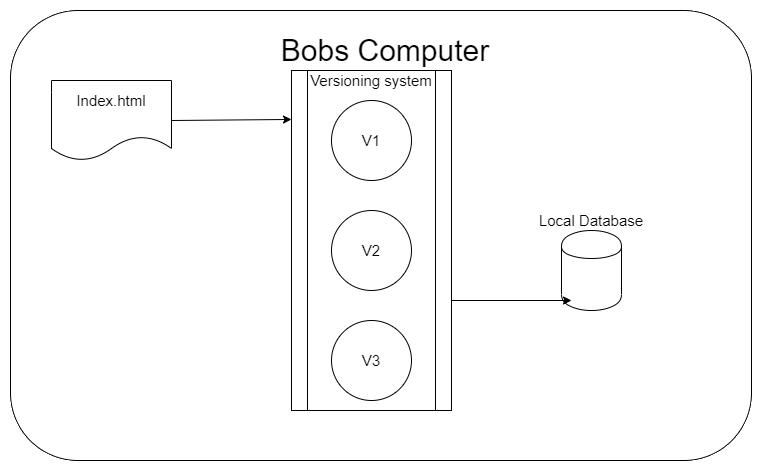
\includegraphics[scale=.3]{LVCS.png}
		\caption[Overzicht structuur Lokale VCS]{Overzicht van de structuur van een Lokale VCS.}
	\end{subfigure}%
	\begin{subfigure}[b]{.5\textwidth}
	\centering
		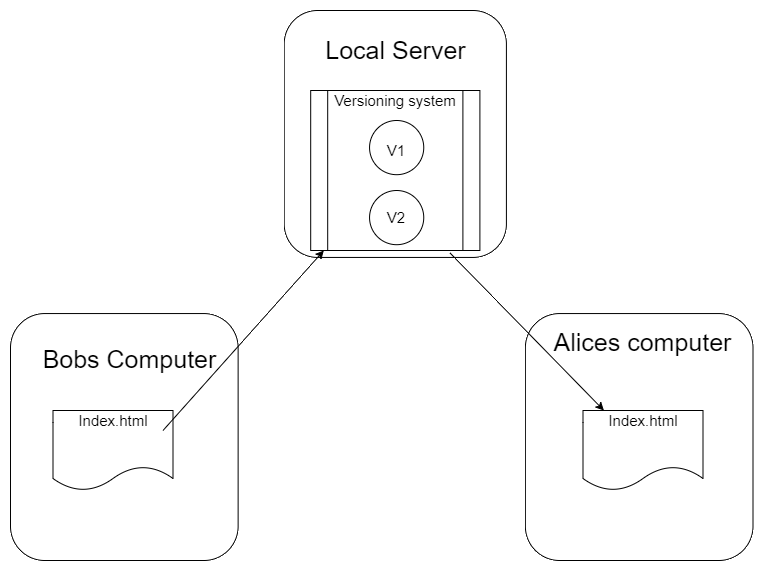
\includegraphics[scale=.3]{CVCS.png}
			\caption[Overzicht structuur CVCS]{Overzicht van de structuur van een CVCS.}
	\end{subfigure}%
	\hfill
	\begin{subfigure}{.5\textwidth}
		\centering
		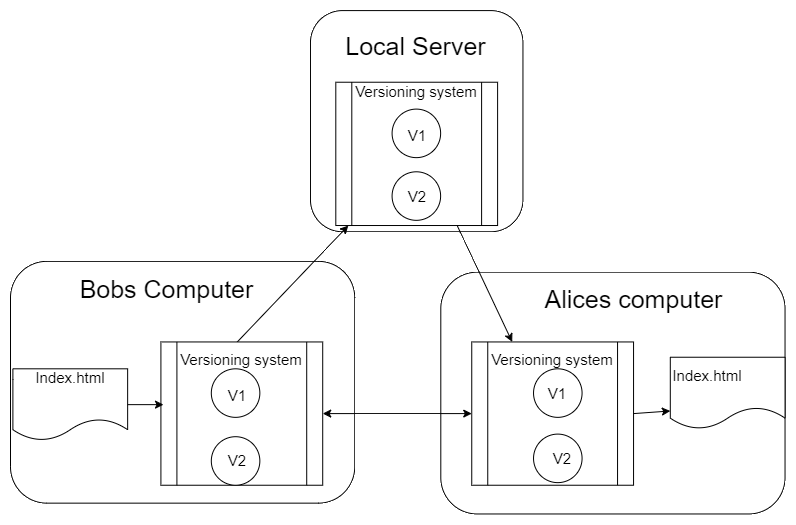
\includegraphics[scale=0.3]{DVCS.png}
	\caption[Overzicht structuur DVCS]{Overzicht van de structuur van een DVCS.}
	\end{subfigure}
	
	\caption[Overzicht types VCS]{Overzicht van de drie types van VCS zoals aangegeven door \textcite{Chacon2014}.}
	\label{fig:TypesVCS}
\end{figure}

	
\subsection{RCS}
\label{sec:RCS}


RCS \textit{(Revision Control System)} is een lokaal versiebeheer systeem. Het werd voor het eerst gedocumenteerd en ontwikkeld in een artikel geschreven door \textcite{Tichy85rcs}.GNU - Een open source besturingssysteem \footnote{GNU is veel meer dan enkel open source. Het GNU project is sterk verbonden met de ideologie en organisatie van de free software foundation (FSF). Meer informatie omtrent deze organisatie en beweging is te vinden op: \url{https://www.fsf.org/}}- gebruikte RCS als vervanging voor het CSSC Systeem \autocite{GNUCSSC}.\\

CSSC was een variant van het SCCS systeem dat ontwikkeld werd aan Bell Labs. SCCS (Source code control system) is een versiebeheer software voor UNIX systemen. Het werd ontwikkeld door \textcite{Rochkind1975}. SCCS was echter niet de enigste op de markt. Zo was er ook nog CA-Panvalet een gepatenteerde oplossing voor Mainframe computers. Toch is RCS de beste keuze om van dichterbij te gaan bekijken. Veel van de concepten waar het gebruik van maakt zijn nog terug te vinden in moderne systemen (zoals GIT). De visie van het project kadert eveneens binnen de algemene filosofie van deze bachelorproef. Het is open source en wordt nog steeds op vrijwillige basis onderhouden. De onderstaande uitleg over RCS is gebaseerd op het originele artikel van \textcite{Tichy85rcs}.\\

Een eerste principe waar het systeem op steunt is een boomstructuur. Een vertrouwd voorbeeld van een boomstructuur is een stamboom. Deze uitleg is gebaseerd op \textcite{Lievens2019}. Een boomstructuur is een collectie van \textbf{toppen} \textit{(in het engels ook wel Nodes genoemd)}. Deze toppen zijn met elkaar verbonden op een hiërarchische manier. Dit wordt bestempeld als een kind-ouder verband. Er zijn twee bijzondere toppen in een boom. Helemaal aan het begin van de boom ligt een top die we ook wel bestempelen als \textbf{wortel} \textit{(Root)}. Deze top heeft geen ouders. Een andere bijzondere top is een \textbf{blad} \textit{(leaf)}. Een blad is een top die geen kinderen heeft. Alle andere toppen worden intermediair genoemd. Elke top heeft een arbitrair aantal kinderen (synoniem van opvolgers) die op hun beurt opnieuw een wortel zijn voor een deelboom. Tot slot speelt binnen RCS ook het concept van \textbf{diepte} een rol. De diepte van de wortel is nul ($d$=0) en elk kind heeft als diepte: 

\begin{equation}
	d_{kind} = d_{ouder} + 1
\end{equation}

Al deze concepten worden ook nog eens grafisch verduidelijkt in de grafiek \ref{fig:tree}.

\begin{figure}[h!]
\centering
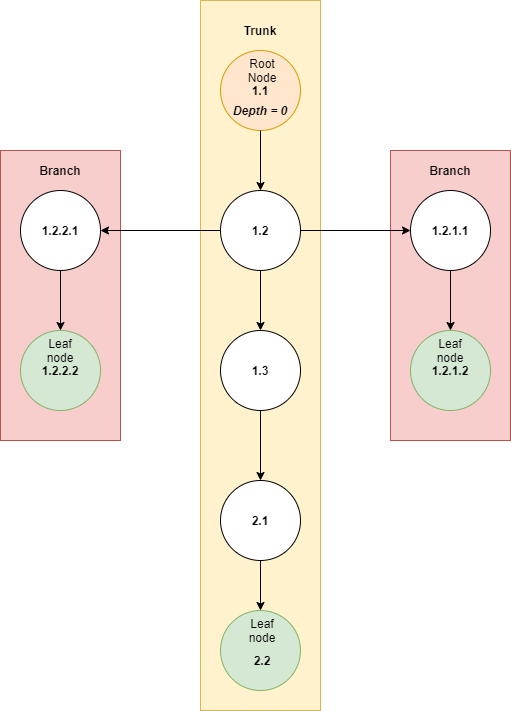
\includegraphics[scale=0.5]{tree1.png}
\label{fig:tree}
\caption[Overzicht concepten boomstructuur]{Een overzicht van alle concepten binnen een boomstructuur waar RCS van gebruik maakt.}
\end{figure}

Er wordt een boomstructuur gebruikt om de verschillende versies en de onderlinge relaties te gaan voorstellen. Stel: Bob en Alice zijn bezig aan de hoofdpagina. Ze hebben elk een aantal wijzigingen aangebracht en willen deze graag met elkaar delen. Ze hebben een terminal verbinding tot een centrale GNU computer. Bob maakt een initiële versie van de pagina en gebruikt vervolgens het commando voor het \textbf{inchecken} (\Verb+ci homepage.html+).Inchecken wordt gebruikt om een nieuwe versie aan te maken. Aangezien dit de eerste versie is wordt er een beschrijving van het project gevraagd. In volgende versies moet men enkel de wijzigingen sinds de vorige versie aangeven. Vervolgens wordt de extensie \textit{.v} toegevoegd (\verb+homepage.html.v+). Het originele bestand zal standaard ook verwijderd worden. Het equivalent voor inchecken bij GIT is het \verb+git Push+ commando.\\

Het bestand krijgt ook een \textbf{versie nummer}. Dit versienummer heeft de vorm: $x_1.x_2$. $x_1$ (ook wel \textit{release} genoemd) staat voor een grote verandering. Bijvoorbeeld het in productie nemen van een nieuwe versie.$x_2$ (\textit{level}) staat voor een kleinere verandering. Een andere manier om $x_2$ te bekijken is de diepte met als wortel de laatste release. Deze manier van versies te bestempelen wordt nog steeds gebruikt. Deze manier is echter niet uniek, \textit{Semantic versioning} is een gekend alternatief. De versie die bob als eerste online heeft gezet krijgt het nummer 1.1. Elke volgende check-in van het bestand zal het level ($x_2$) met één gaan verhogen. De volgende versie wordt dus 1.2. Het release nummer ($x_1$) wordt manueel verhoogd doormiddel van de \textit{-r} optie bij check-in. Bij branches is er ook nog spraken van $x_3$ en $x_4$ zie \ref{par:branches}. Dit concept bestaat in Git onder de vorm van \textit{tags} (\ref{sec:GIT}).\\

Er is nu een bestand onder de vorm \Verb+homepage.html.v+ maar hoe kan Alice nu dit bestand gaan aanpassen? Alice gaat het bestand moeten \textbf{uitchecken} door middel van het commando  \verb+co homepage.html+. Op die manier kan de nieuwste versie van het bestand opgevraagd worden. Vervolgens worden de wijzigingen aangebracht en gaat het bestand door Alice weer worden ingecheckt. Met de \textit{-r} optie kunnen we een specifieke versie gaan ophalen. Het equivalent van \verb+co+ binnen git is het concept van \verb+pullen+.\\

\begin{wrapfigure}{r}{0.5\textwidth}
\label{fig:deltas}
\begin{center}
  	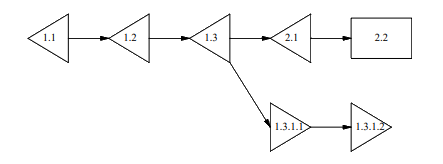
\includegraphics[scale=0.6]{deltas.png}
\end{center}
\caption[Voorbeeld van deltas.]{Een voorbeeld van deltas.De Trunk bevat een series van achterwaardse deltas terwijl alle branches enkel voorwaardse deltas bevatten. Grafiek afkomstig uit \textcite{Tichy85rcs}}
\end{wrapfigure}

Hoe weet RCS echter wat het verschil is tussen versie 1.1 en 1.2? Een eerste naïeve oplossing zou zijn om alle versies van het bestand afzonderlijk te gaan bijhouden. Dit vraagt echter veel opslagruimte. RCS gebruikte voor dit probleem het concept van \textbf{deltas}. Een delta is een bestand dat bijhoud welke lijnen van je bestand concreet veranderd zijn tussen de versies. Heeft men dus één lijn verwijderd in een bestand zal de delta maar één regel gaan opnemen \footnote{De delta wordt opgebouwd aan de hand van het GNU commando diff \url{https://www.gnu.org/software/diffutils/}}. Er zijn twee types van deltas: \textbf{voorwaardse deltas}en \textbf{achterwaardse deltas}. Bij het in-checken van een nieuwe versie zal de vorige versie worden vervangen door een achterwaardse  delta. Zit men momenteel op versie 1.3 en  vraagt men versie 1.2 dan zal de achterwaardse delta van versie 1.2 worden toegepast op versie 1.3. Voorwaardse deltas komen aanbod in het gedeelte over branching (\ref{par:branches}).Dit concept wordt ook nog eens verduidelijkt in grafiek \ref{fig:deltas} .\\

Door dit principe van inchecken en uitchecken hebben we dus al een werkend systeem. Er is echter wel nog een probleem stel dat Bob en Alice samen versie 1.2 hebben uitgecheckt, ze brengen alle twee wijzigingen aan en willen in-checken. Wie krijgt voorrang? Dit probleem wordt opgelost door het concept van \textbf{sloten}(engels=lock). Op het moment dat  Bob zijn versie gaat uitchecken kan hij deze versleutelen (door middel van de \textit{-l} optie bij het co commando). Hierdoor kan niemand anders dan Bob een nieuwe versie gaan in-checken \footnote{Andere gebruikers kunnen echter wel nog de versleutelde versie gaan bekijken}. Het bestand ligt dus vast tot Bob het slot vrijgeeft door een nieuwe versie te gaan publiceren \footnote{In sommige gevallen kan het slot ook worden 'geforceerd' mocht Bob bijvoorbeeld ziek vallen}. Deze manier van werken heeft duidelijk een groot aantal nadelen. Alice is verplicht om te wachten op Bob zijn nieuwe versie alvorens ze veranderingen kan maken. Git zal dit probleem anders gaan aanpakken door middel van het introduceren van \textit{Merges}.De veranderingen die Alice aanbrengt en de verandering van bob zouden door merges worden samengevoegd tot één nieuwe versie.\\

\label{par:branches}

\subsubsection{Opmerkingen}
In het originele artikel wordt de klemtoon gelegd op het onderling delen van de verschillende versies. Hierdoor kan men de indruk krijgen dat er een centrale server betrokken is. Dit is niet het geval. De software is ontworpen om op één besturingssysteem uitgevoerd te worden. Volgens \textcite{Debian2020} is GNU aangezien het gebaseerd is op UNIX een \textit{multi-user os}. Dat wilt zeggen dat meerdere gebruikers het systeem tezelfdertijd kunnen gebruiken door middel van een terminal connectie. Hierdoor kan men onderling de bestanden gaan delen ondanks dat men niet gaat werken in een CVCS -zie \ref{sec:CVCS}-.

\subsection{CVCS}
\label{sec:CVCS}

\subsection{GIT}
\label{sec:GIT}
